

\chapter{Chatbot and AI integration}
\section*{Introduction}
\addcontentsline{toc}{section}{Introduction}
The VitamiNurse app stands out from other traditional nutrition apps through its advanced use of artificial intelligence .

In addition to the use of the sentence transformer model to generate vector embeddings  in the recommendation system  discussed earlier, this section introduces two key AI components: a product analysis system and an AI assistant.

  By acting as a nutrition coach, this AI assistant understands health status and preferences of each user. The integration of this chatbot transforms static product recommendations into an interactive dialogue system that is available 24/7 to answer their questions and provide advice.

The following sections detail the architecture and functionality of these AI systems within the VitamiNurse mobile app.

\section{Advanced scan system with AI analysis }

Instead of showing large amounts of raw product data, VitamiNurse uses AI to interpret the product after scanning its barcode.  Through the combination of detailed nutritional information, user health profiles, and AI reasoning based on prompts, the VitamiNurse app provides customized nutritional guidance in a way that traditional tools cannot. The result is a highly interactive and user-friendly experience that transforms a simple scan into an informed decision-making process.

\begin{figure}[H]
    \centering
    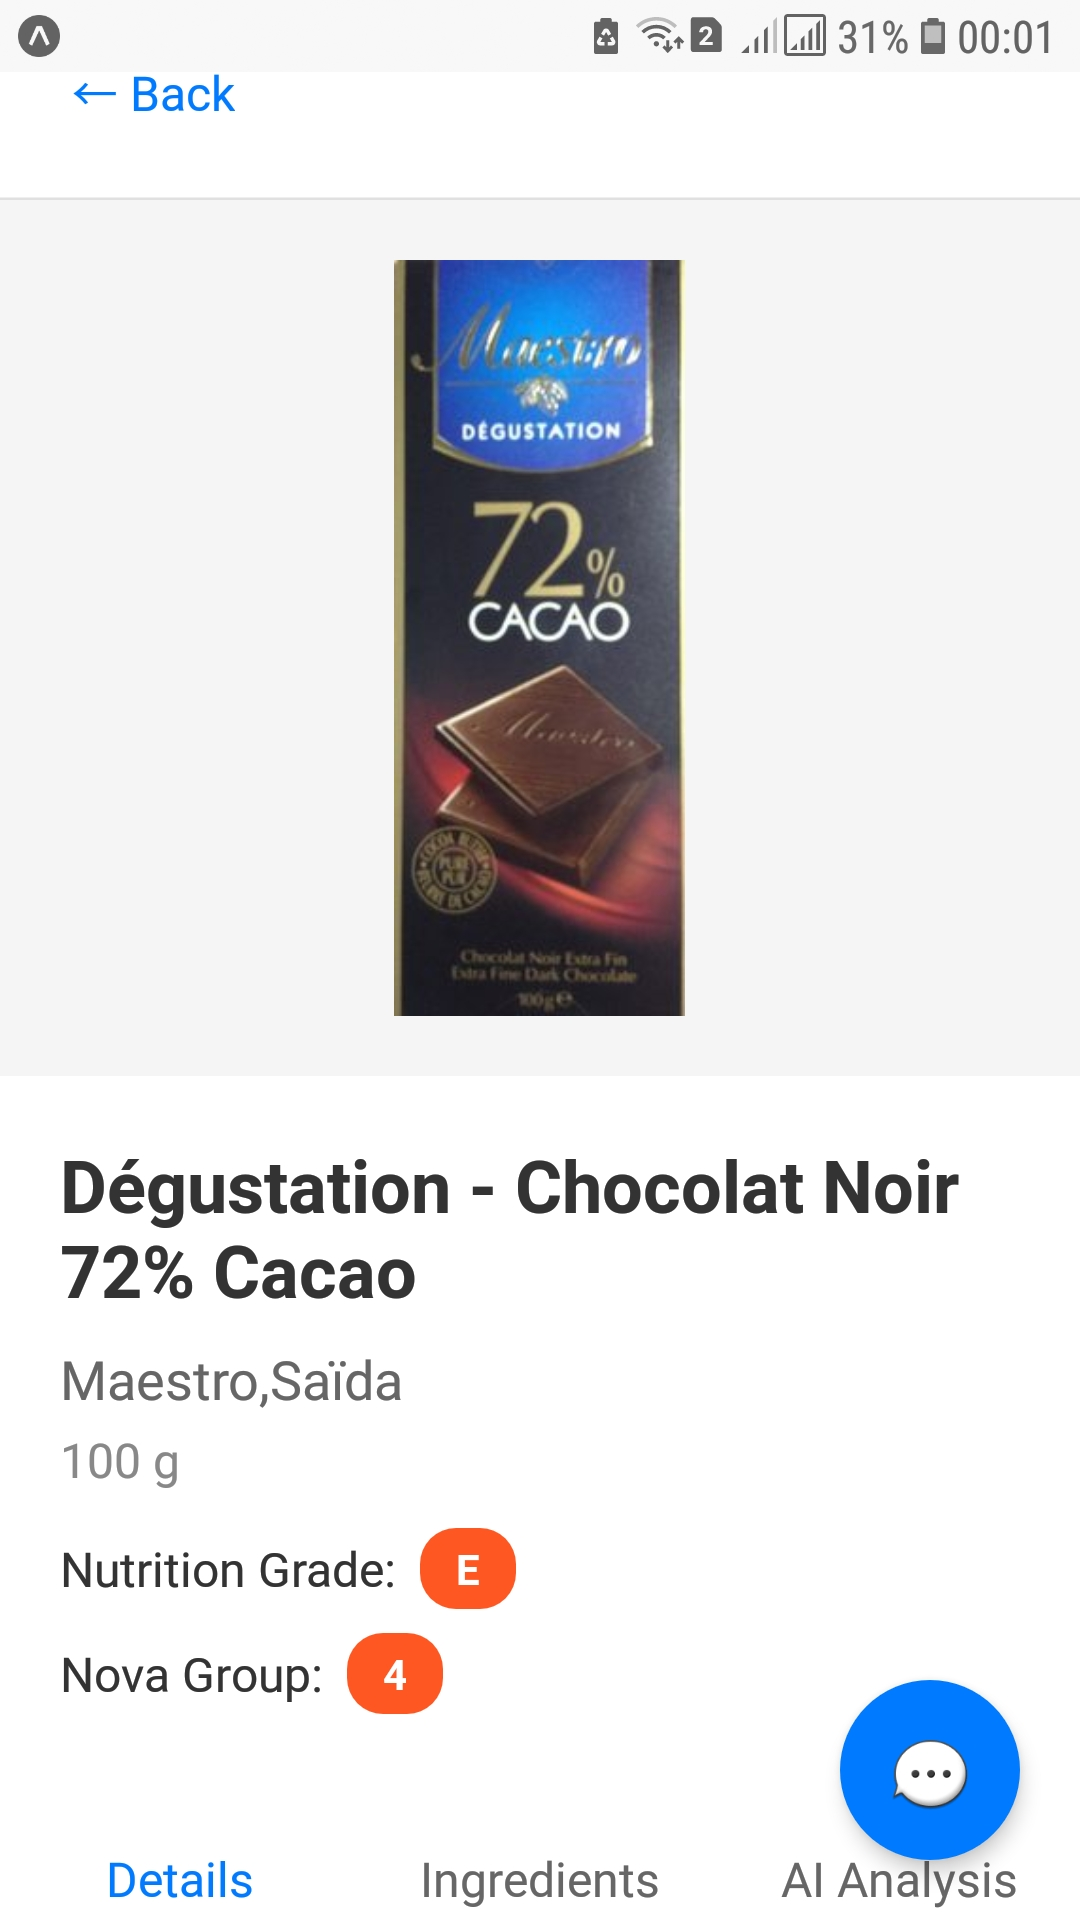
\includegraphics[width=0.22\textwidth]{images/Screenshot_20250920-000112_chocolat_noir.jpg}
    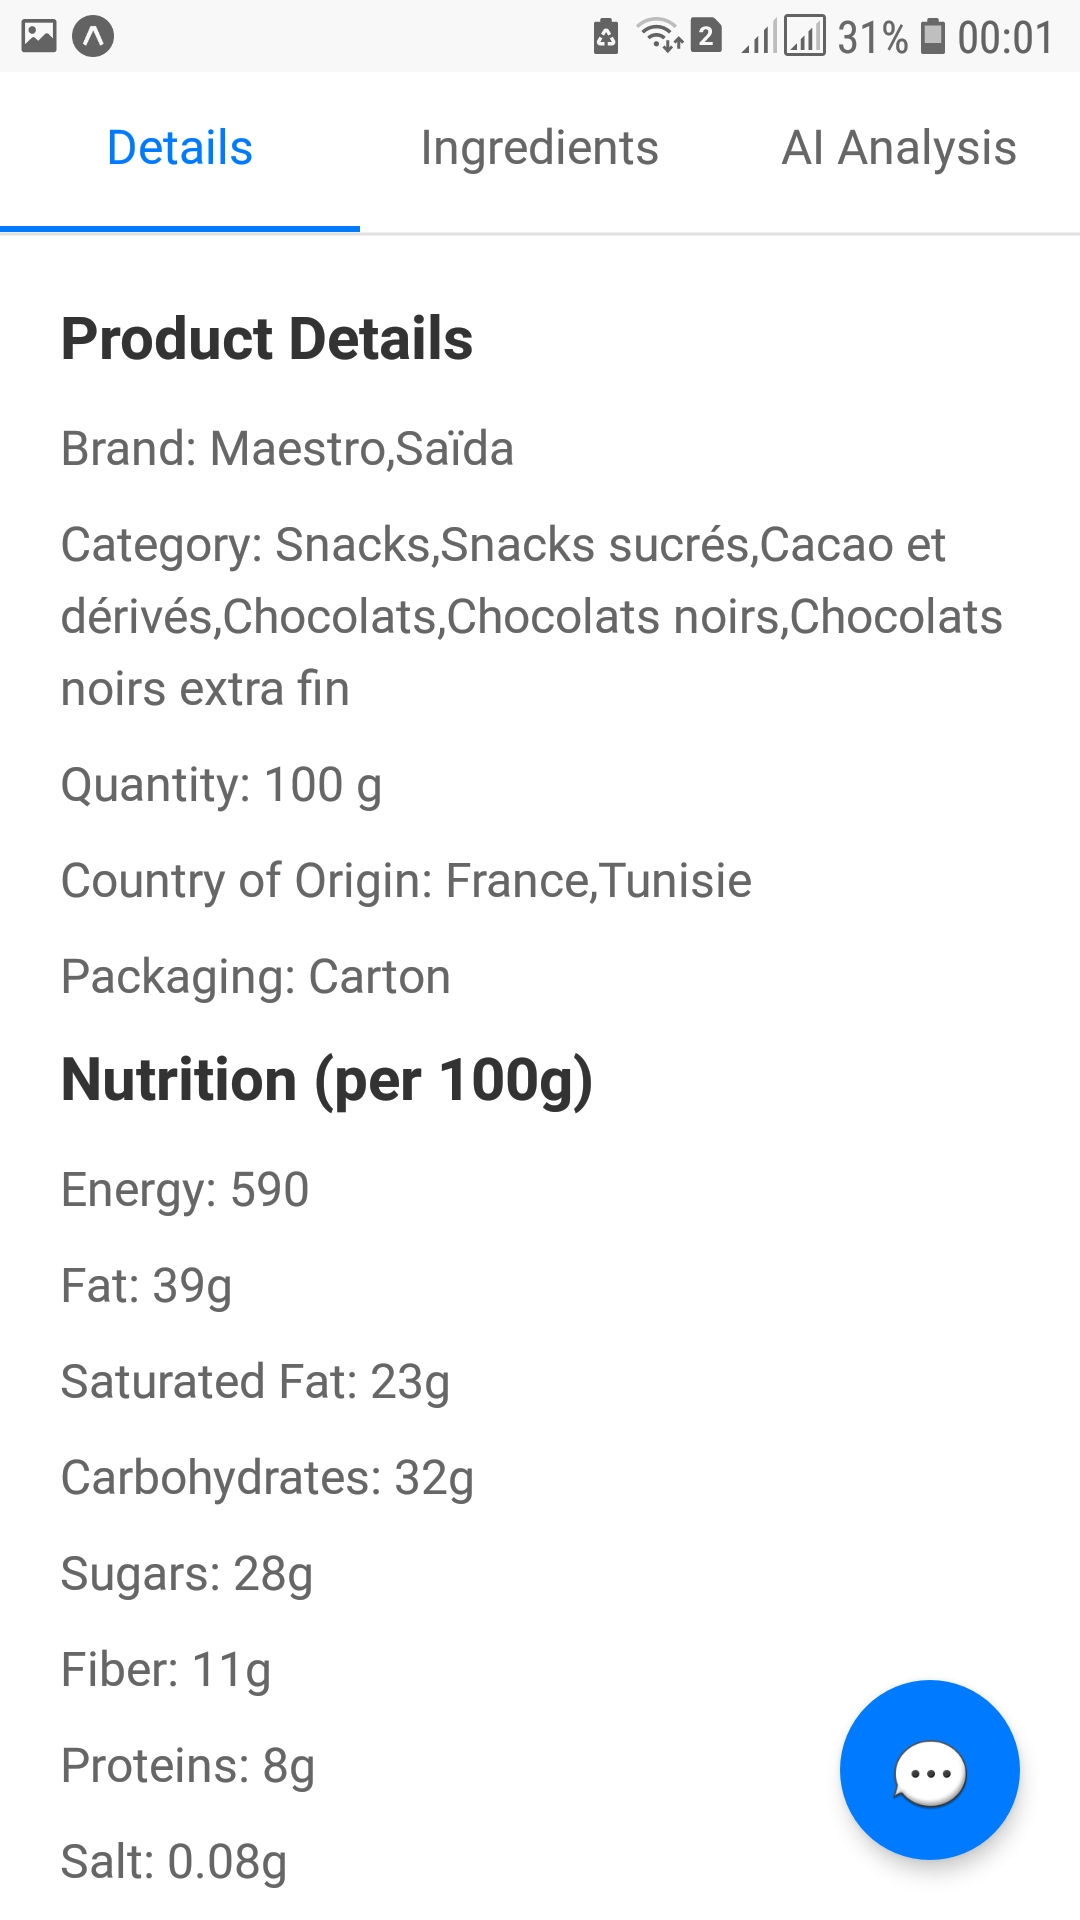
\includegraphics[width=0.22\textwidth]{images/Screenshot_20250920-000118_chocolat_noir.jpg}
    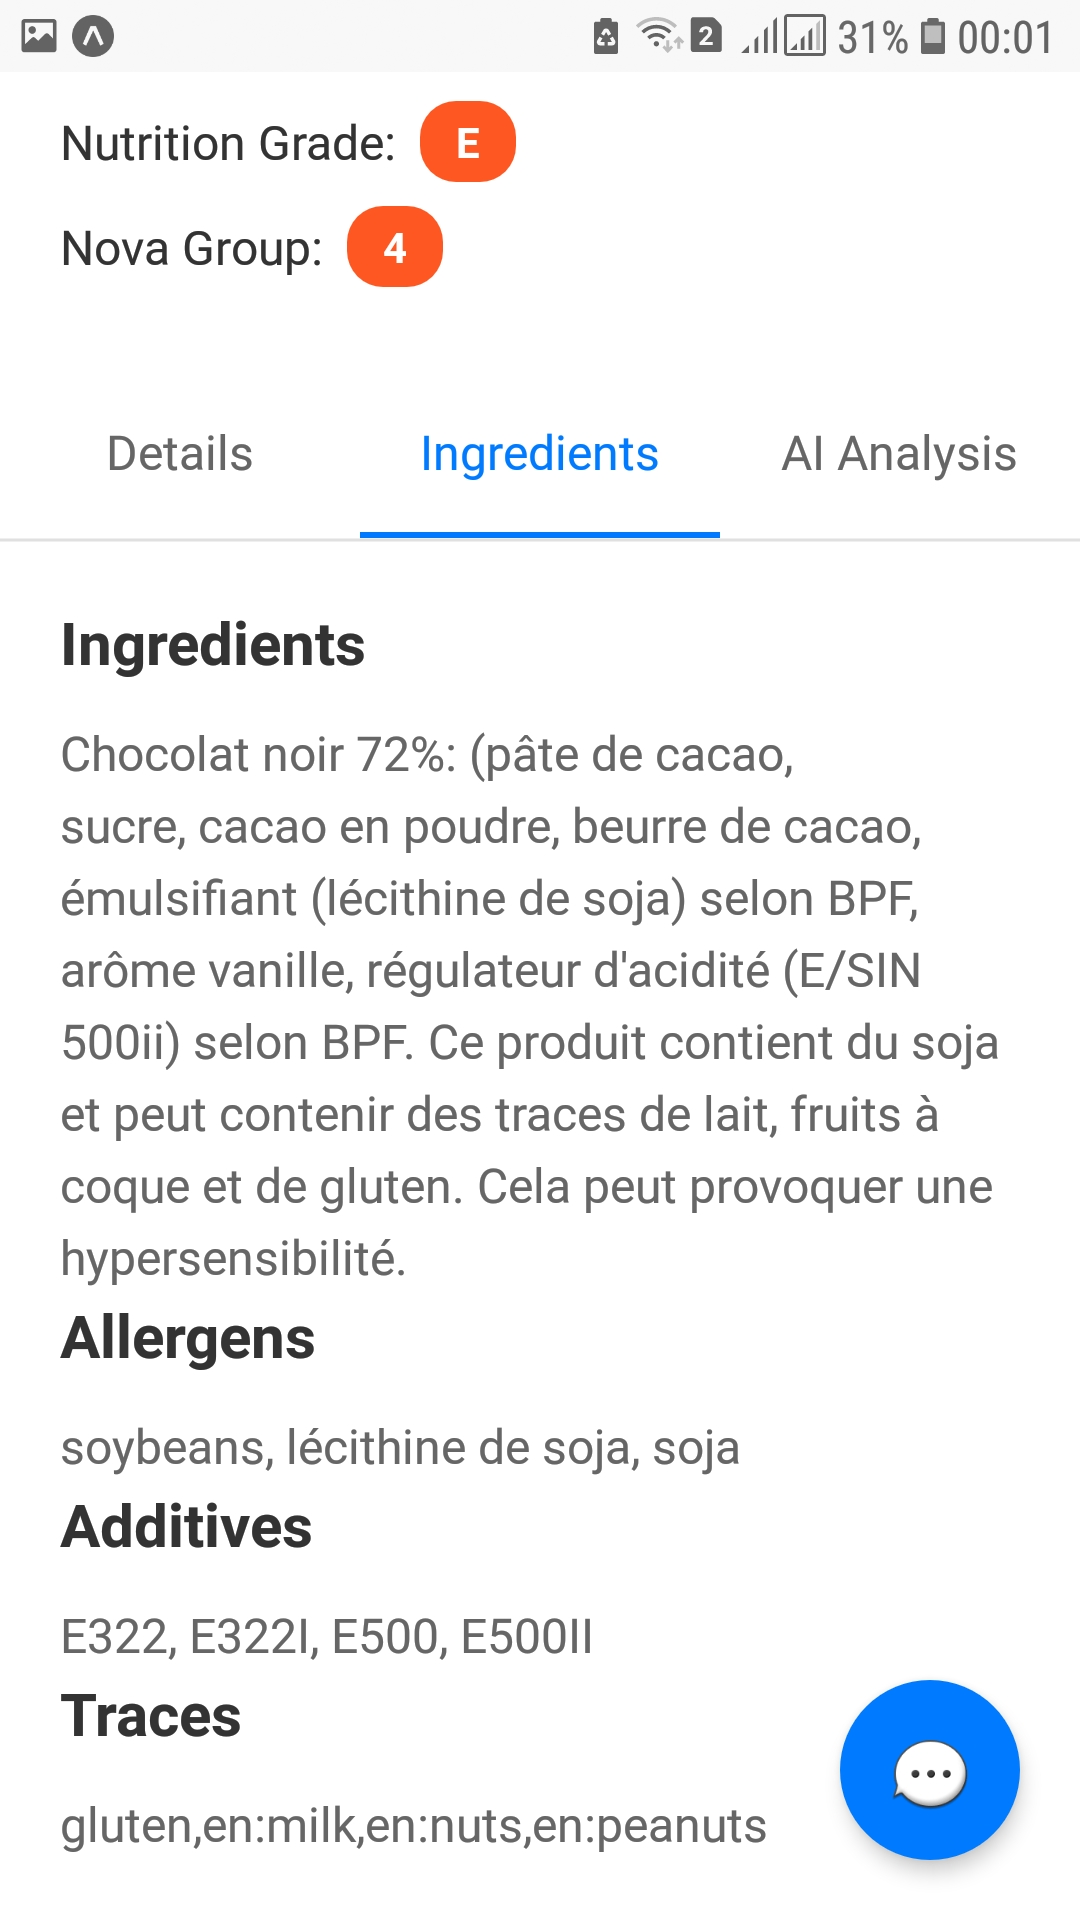
\includegraphics[width=0.22\textwidth]{images/Screenshot_20250920-000124_chocolat_noir.jpg}
    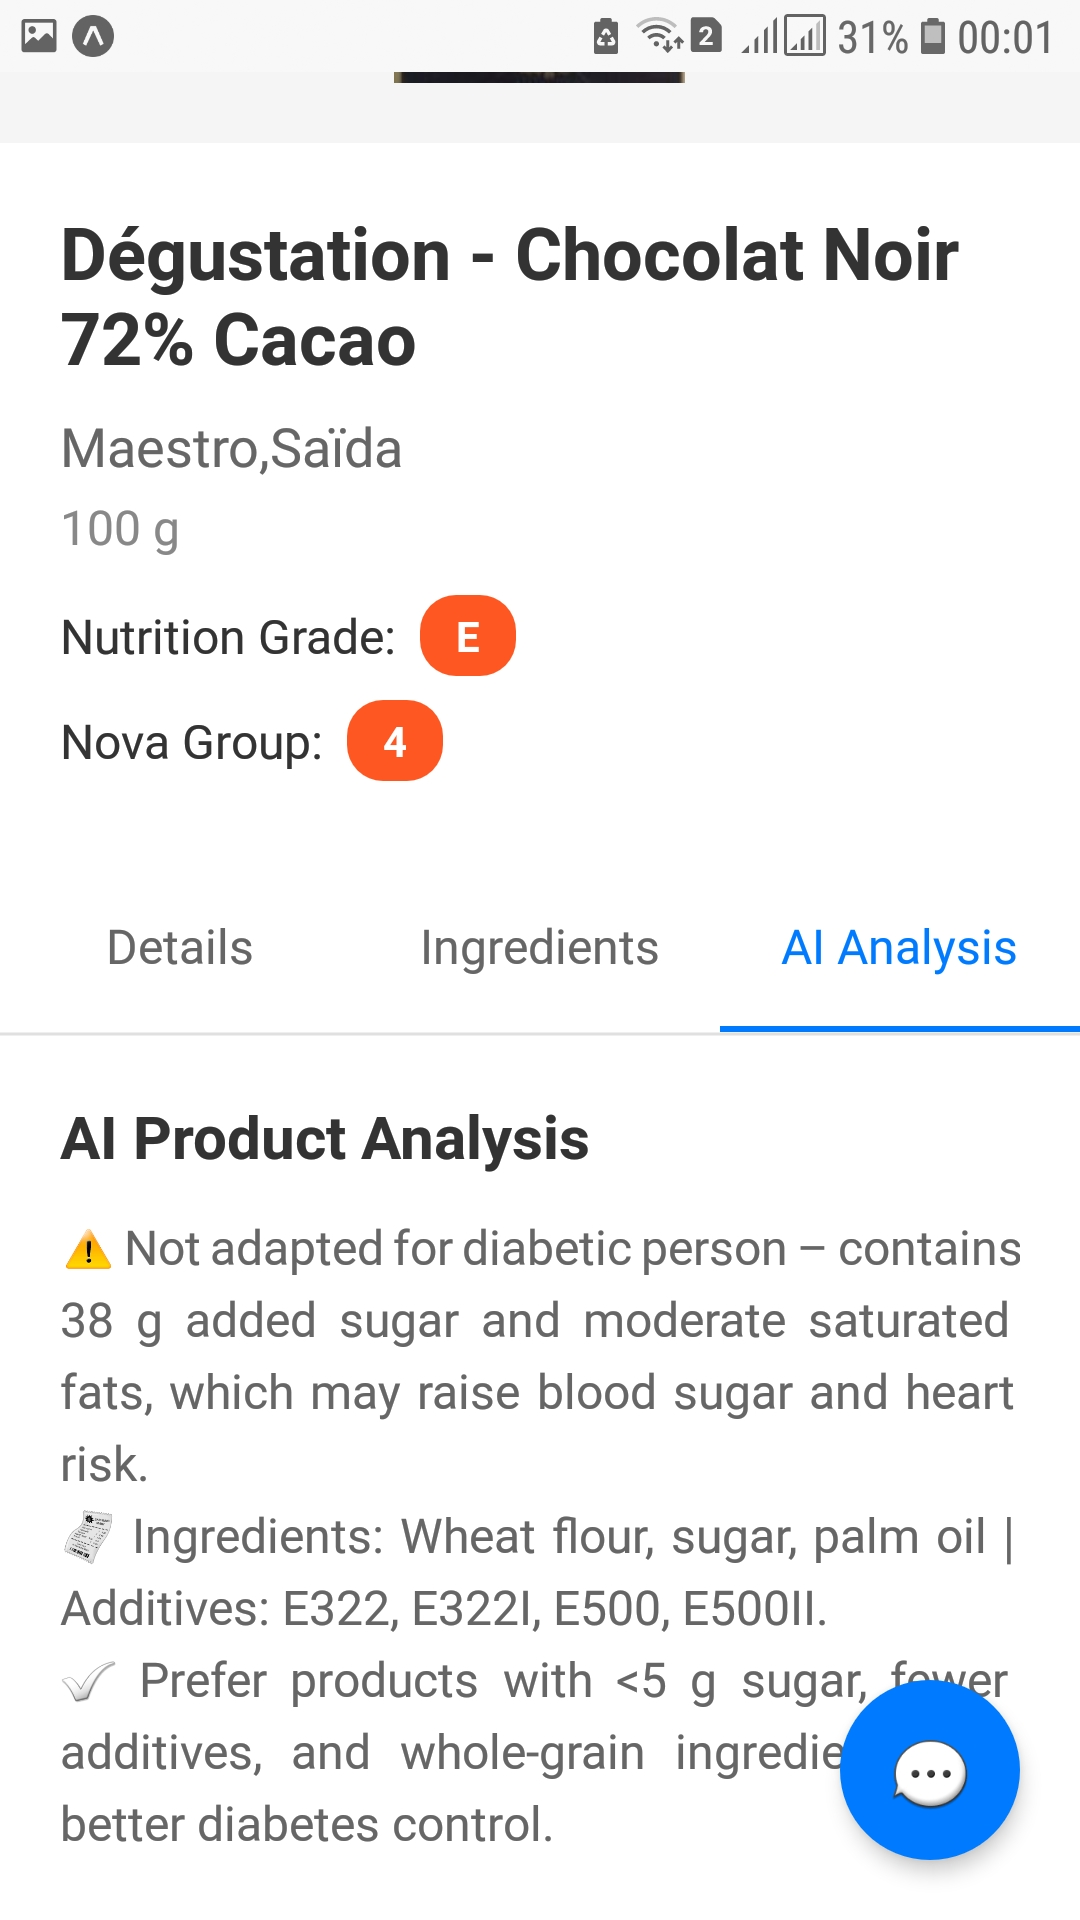
\includegraphics[width=0.22\textwidth]{images/Screenshot_20250920-000137_chocolat_noir.jpg}
    \caption{Advanced product evaluation with AI analysis}
    \label{fig:advanced_AI_evaluation}
\end{figure}

\subsection{Large Language Models (LLMs)}
Large language models are advanced deep learning models trained on vast amounts of texts in order to understand and generate human-like language. 
According to AWS, large language models are very large deep learning models that are pretrained on vast amounts of data\cite{awsLLM}. These models, such as GPT-4 and BERT, have demonstrated remarkable capabilities in differents tasks  significantly advancing the field of NLP like text completion, translation, and specially question-answering, which is required in the  AI assistant of VitamiNurse.

\subsection{Prompt Engineering for AI Analysis}
\par In addition to the details of the product that appear on the screen after scanning the barcode, we added an AI analytics system to provide a concise and personalized conclusion.
 The generative AI capabilities of our system are powered by a popular pretrained LLM, which is ChatGPT-4, to build accurate and relevant responses.
 \par The system uses well structured prompts to guide the AI during the product evaluation.
The following code illustrates how each prompt integrates essential product information with user-specific data, including health conditions and allergies, to determine the suitability of the product for the user profile.
 \begin{center}
    \begin{figure}[H]
    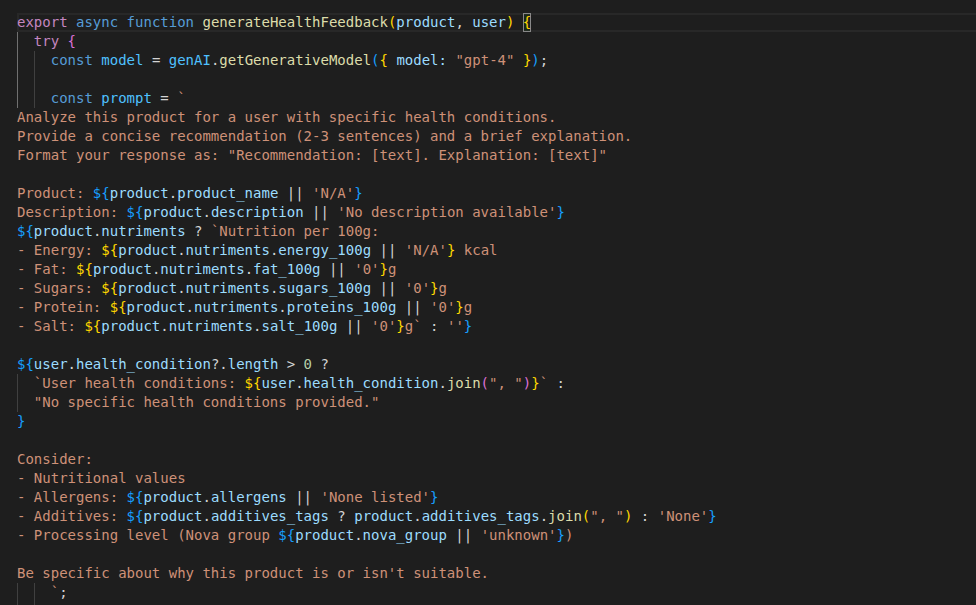
\includegraphics[width=0.9\textwidth]{images/prompt_engineering.png}
    \caption{Prompt Engineering Using GPT-4} 
    \label{fig:Prompt_Engineering}
\end{figure}
\end{center}

\subsection{System operation in VitamiNurse}
The AI analysis system in VitamiNurse integrates a product scanning feature with real-time health feedback, powered by a combination of external APIs, a MongoDB database, and the ChatGPT-4 model. Users can scan a barcode (EAN) to retrieve detailed nutritional information, which is cross-referenced with their health profile stored in the \texttt{users} collection. The system first checks our database for existing product data. If it is unavailable, it fetches data from the OpenFoodFacts API and caches it for future use.

The AI then processes these data alongside user health conditions to generate personalized feedback: \textbf{Is this product suitable or not, and why?}

\par The following picture illustrates how the user sees the details of the scanned product and generated health feedback by the AI analytics system:

\begin{figure}[H]
    \centering
    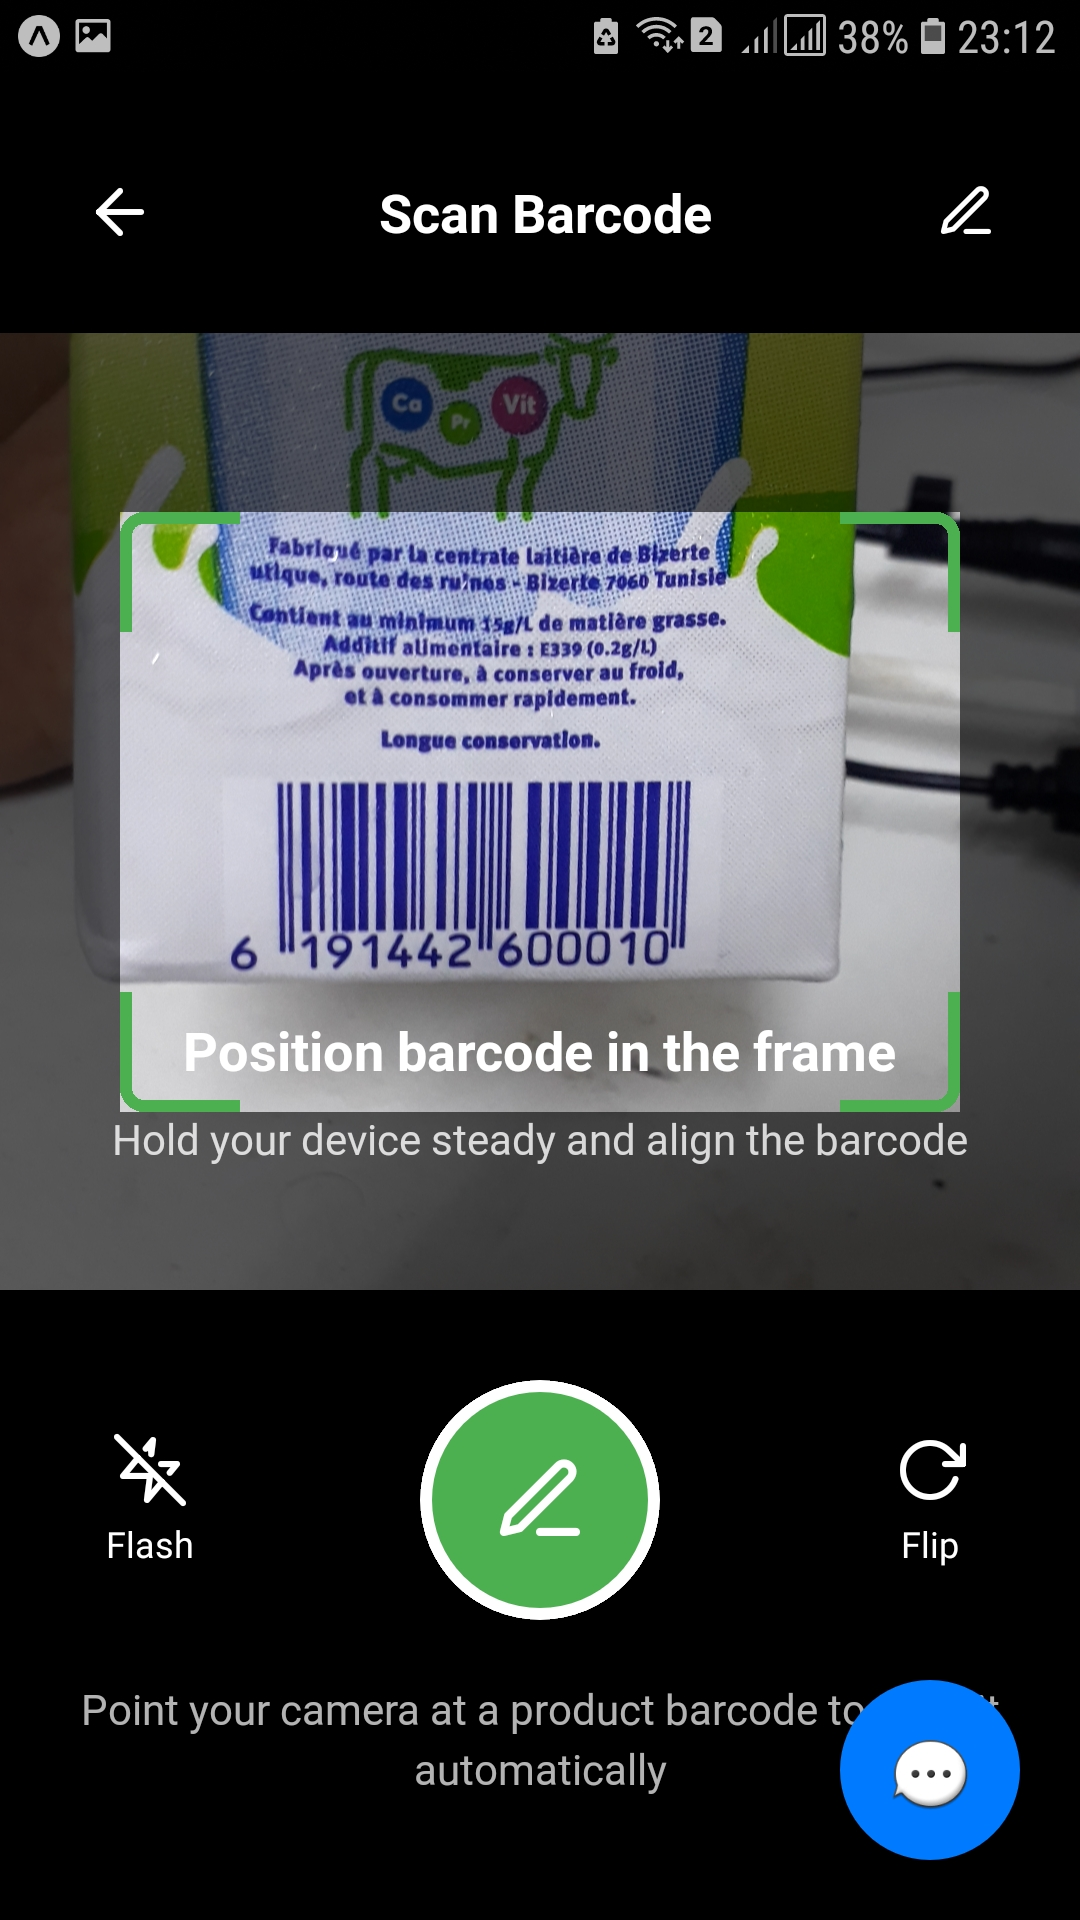
\includegraphics[width=0.22\textwidth]{images/Screenshot_20250919-231229_SCANN_barecode.jpg}
    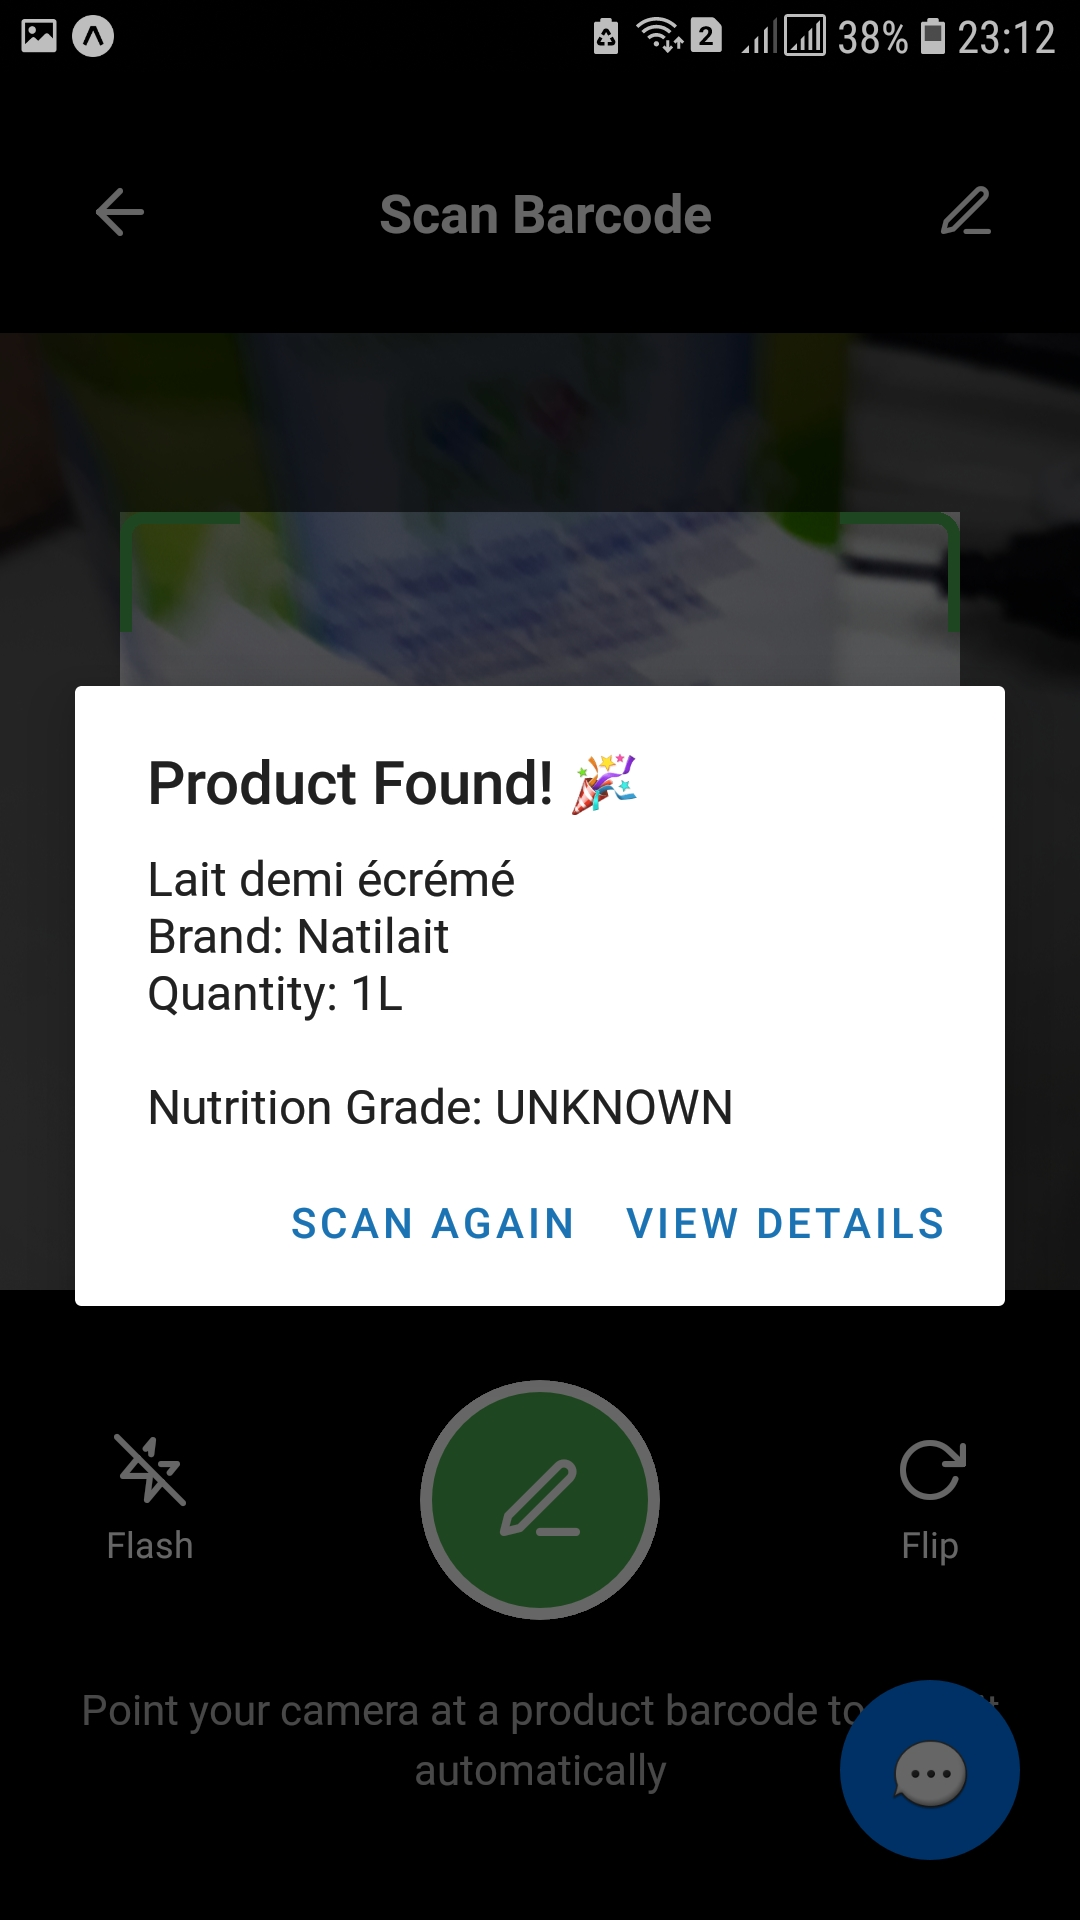
\includegraphics[width=0.22\textwidth]{images/Screenshot_20250919-231233_Scann_success.jpg}
    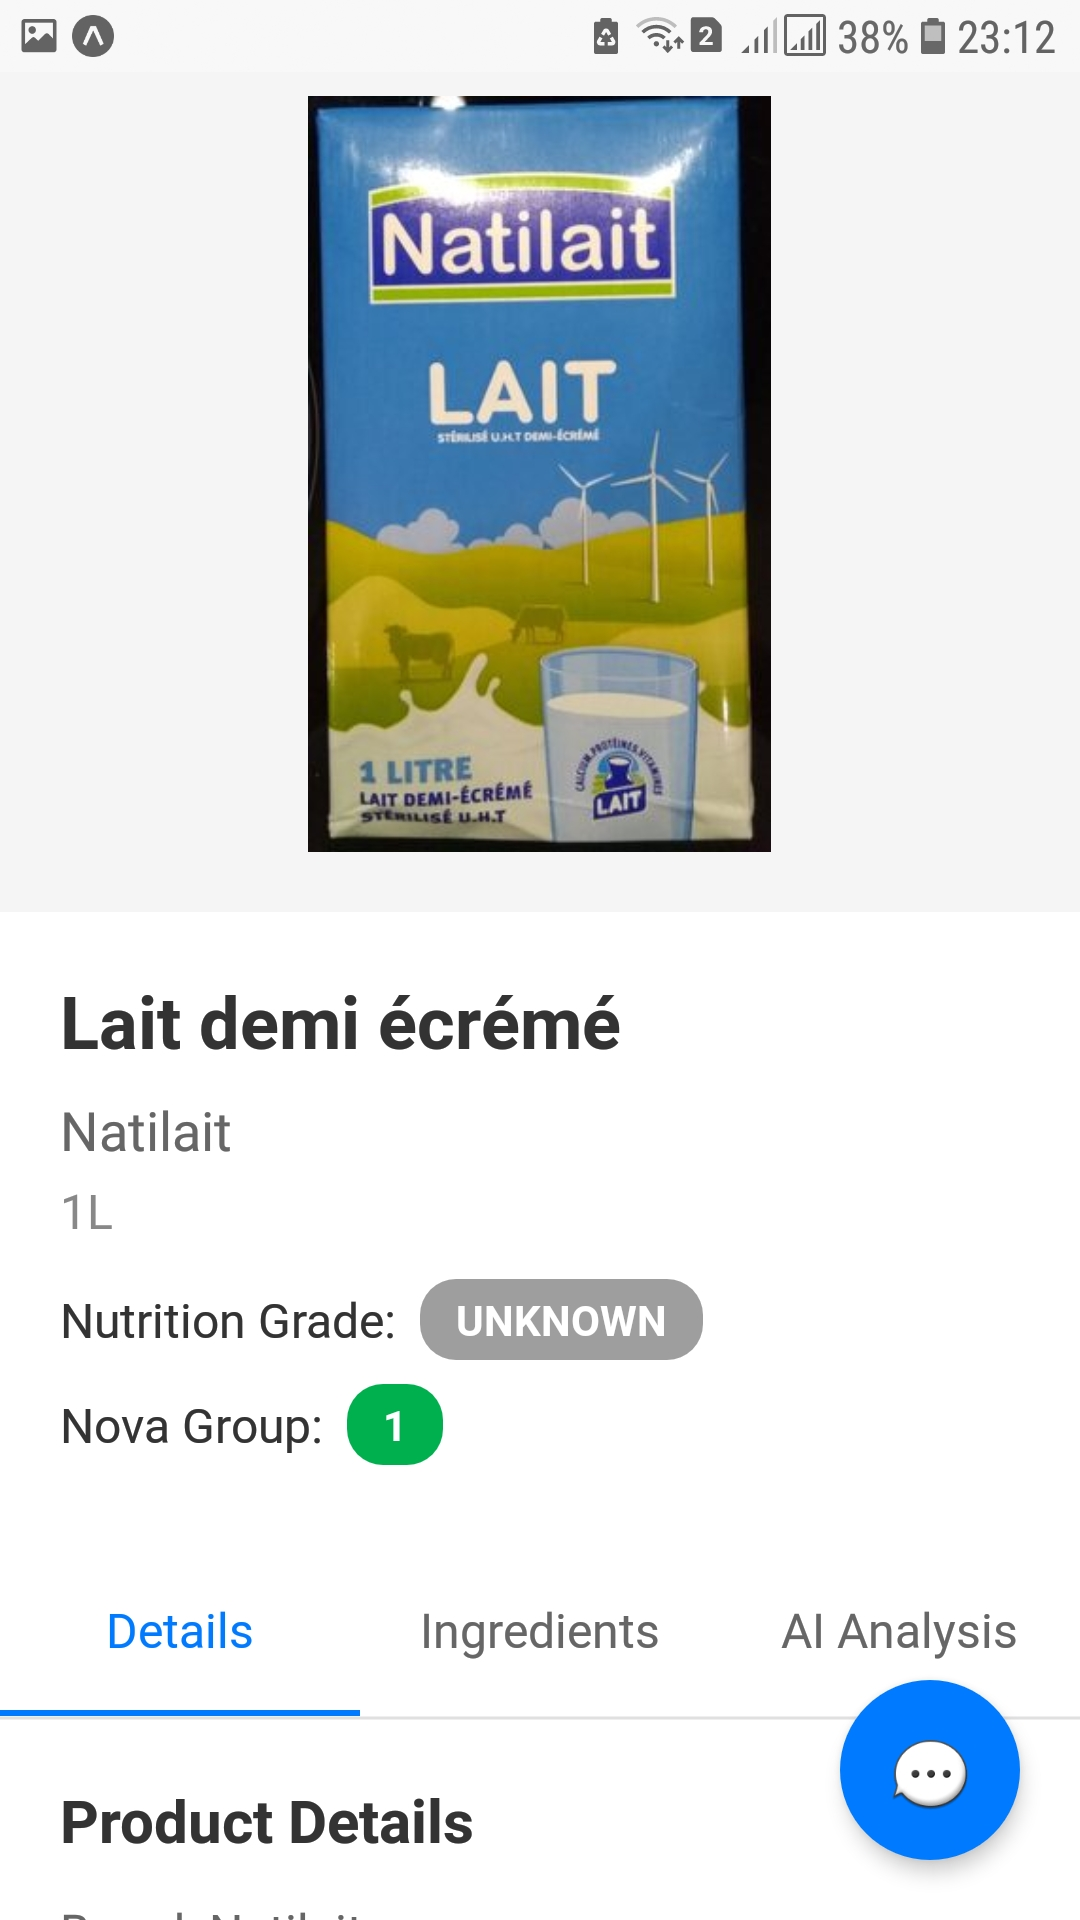
\includegraphics[width=0.22\textwidth]{images/Screenshot_20250919-231251_SCANN-end.jpg}
    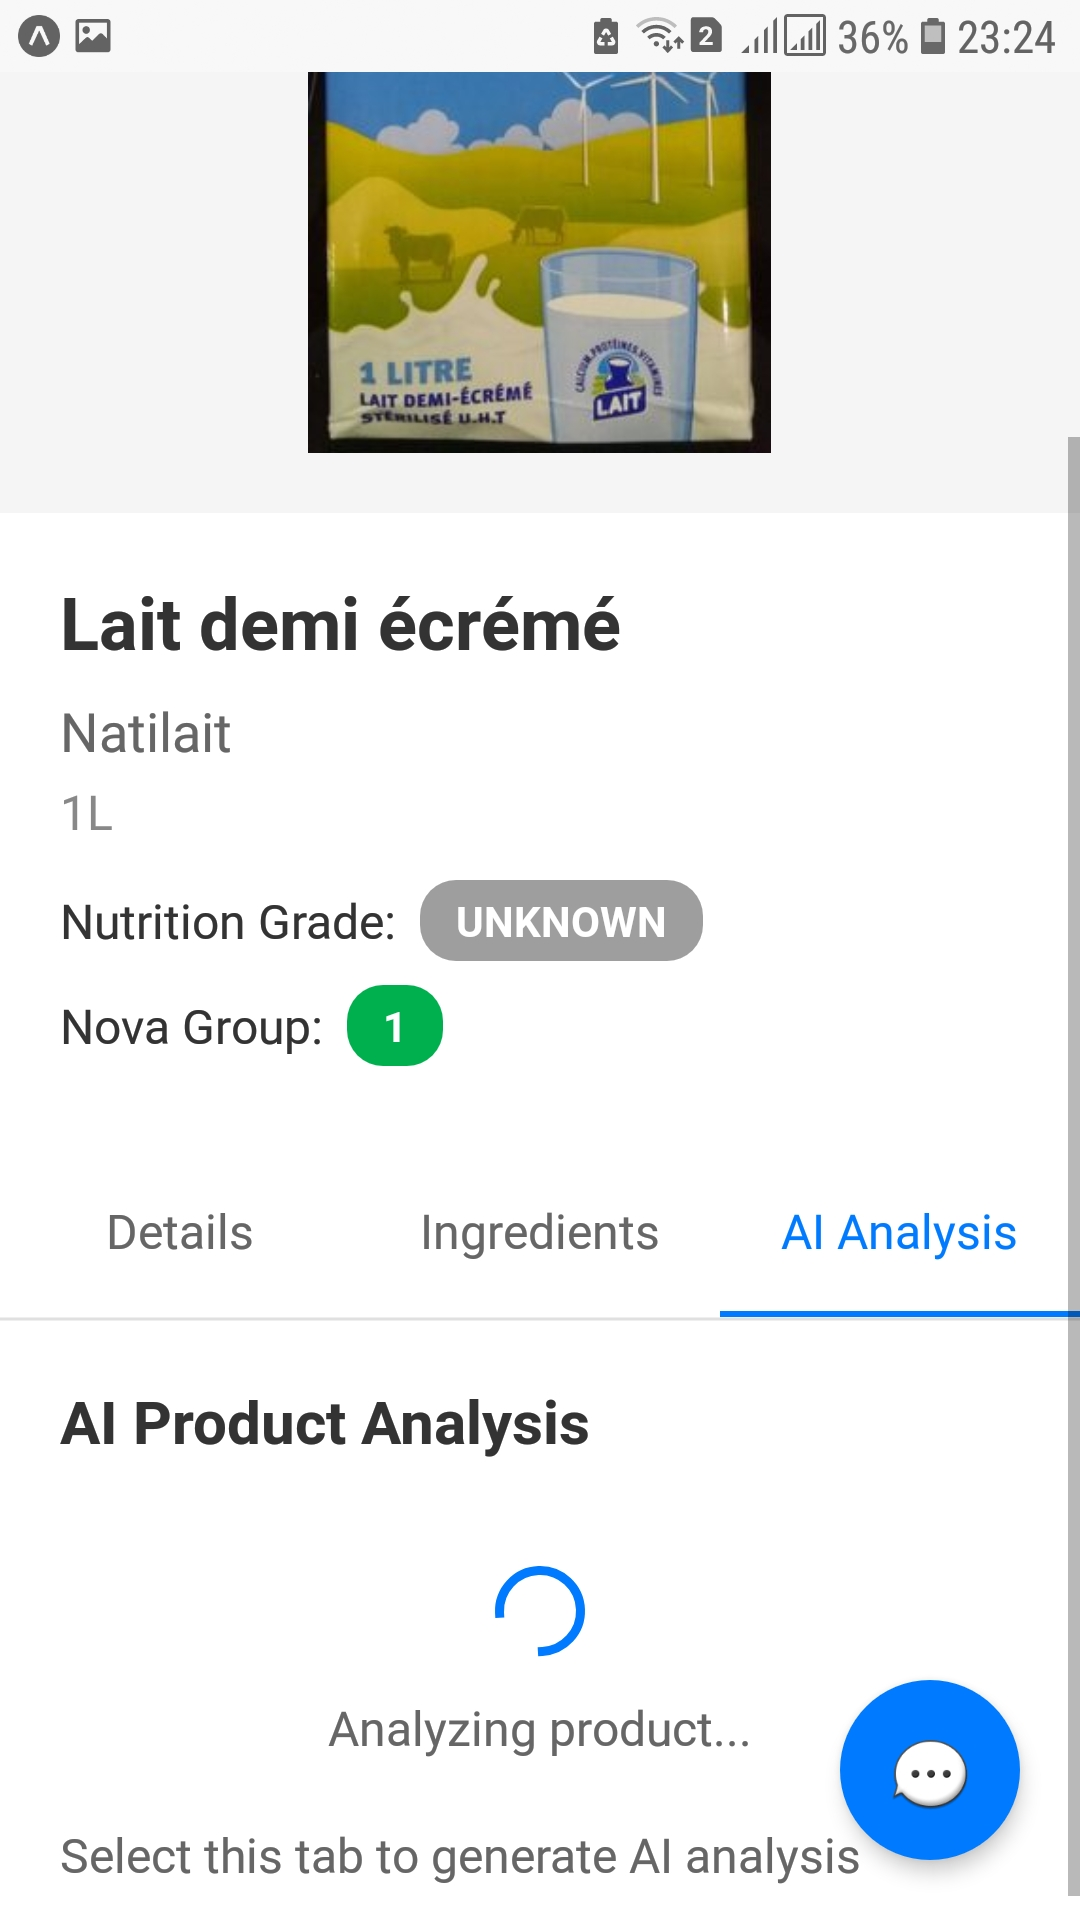
\includegraphics[width=0.22\textwidth]{images/Screenshot_20250919-232403_SCANN_AI_analysis.jpg}
    \caption{Scanned product details and AI nutrition evaluation}
    \label{fig:natilait_screenshots}
\end{figure}

\section{The AI Assistant}
The VitamiNurse AI Nutrition Assistant represents a new generation of personalized nutritional advice and data analysis, all within a coherent conversational interface. It successfully integrates a recommendation engine into a sophisticated LangChain-powered architecture. The system demonstrates how parallel intent processing, dynamic profile management, and AI-generated content can create a comprehensive and personalized nutritional guidance tool.

\subsection{System Architecture}
The architecture of the Nutrition Assistant is designed for modularity, scalability, and maintainability. Figure~\ref{fig:chatbot Architect} outlines this three-tier architecture, consisting of the user mobile interface, backend server, and AI/data layer.
 This separation ensures that improvements in one layer can be implemented without disrupting other components of the system. The conversational capabilities of this intuitive chatbot are tightly integrated with a persistent memory framework in order to recall previous user interactions and adapt recommendations over time.  
 \begin{center}
    \begin{figure}[H]
    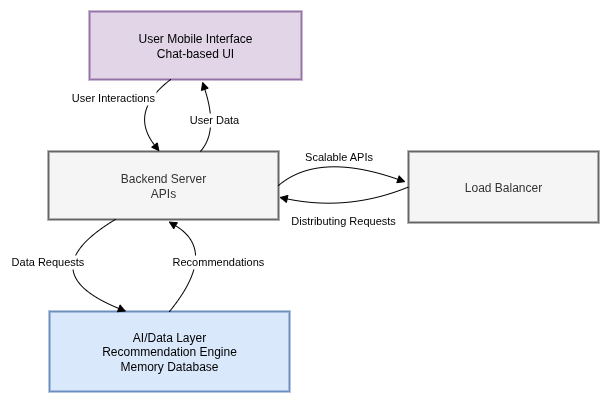
\includegraphics[width=0.7\textwidth]{images/Chatbot_arch.png}
    \caption{Chatbot Architecture} 
    \label{fig:chatbot Architect}
\end{figure}
\end{center}

\subsubsection{User Mobile Interface}
The mobile interface functions as the central interaction point for users engaging with the VitamiNurse assistant, supporting key features such as conversational dialogue and product scanning.
When a user scans a product barcode or types a question, the interface sends a structured request to the backend, which in turn invokes the AI modules for analysis. 
\par The design emphasizes simplicity and readability, ensuring that even complex nutritional assessments are communicated in concise, easy-to-understand language. This is achieved through the adoption of a fixed \texttt{“Recommendation + Explanation”} format, which the AI adheres to when generating responses. The application returns the scanned product's details and nutritional breakdowns as well as AI analysis for this product, making the experience both informative and engaging.
\begin{center}
\begin{figure}[H]
\centering
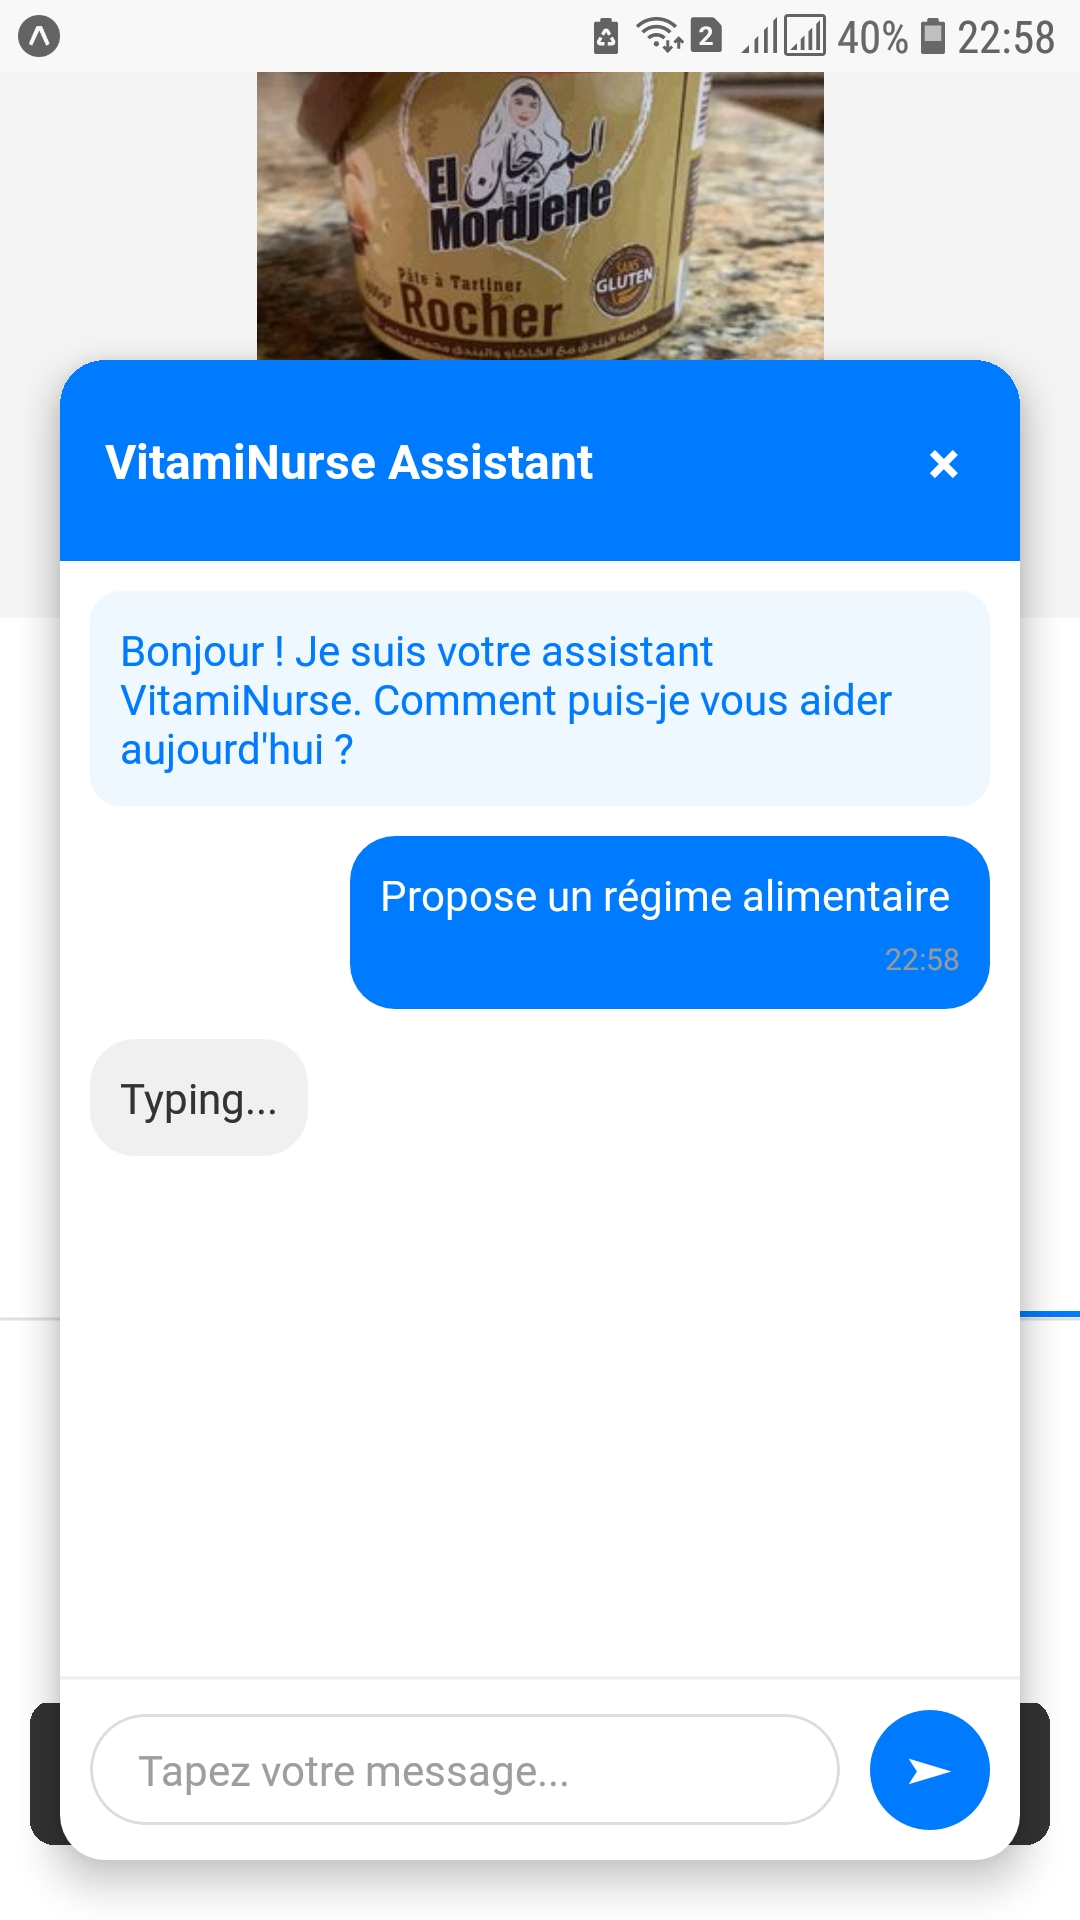
\includegraphics[scale=0.11]{images/Screenshot_20250919-225837_chatbot.jpg}
\caption{AI assistant chat interface}
\label{fig:chat_interface}
\end{figure}
\end{center}

\subsubsection{Backend (FastAPI Server)}
The backend, developed using the \texttt{FastAPI} framework, functions as the system’s control hub. It is responsible for orchestrating communication between the mobile interface, AI reasoning layer, and data storage modules. Upon receiving a request, the backend validates the input, retrieves relevant product data from the nutritional database, and enriches it with user-specific profile information. It then constructs a prompt to be sent to the large language model (LLM), ensuring that all relevant dietary constraints and health conditions are explicitly included. The backend also maintains user session management, conversation history storage, and security protocols for handling sensitive health-related information. Thanks to FastAPI’s asynchronous capabilities, the backend can handle concurrent user requests with minimal latency, which is crucial for providing real-time responses.
 \begin{center}
    \begin{figure}[H]
    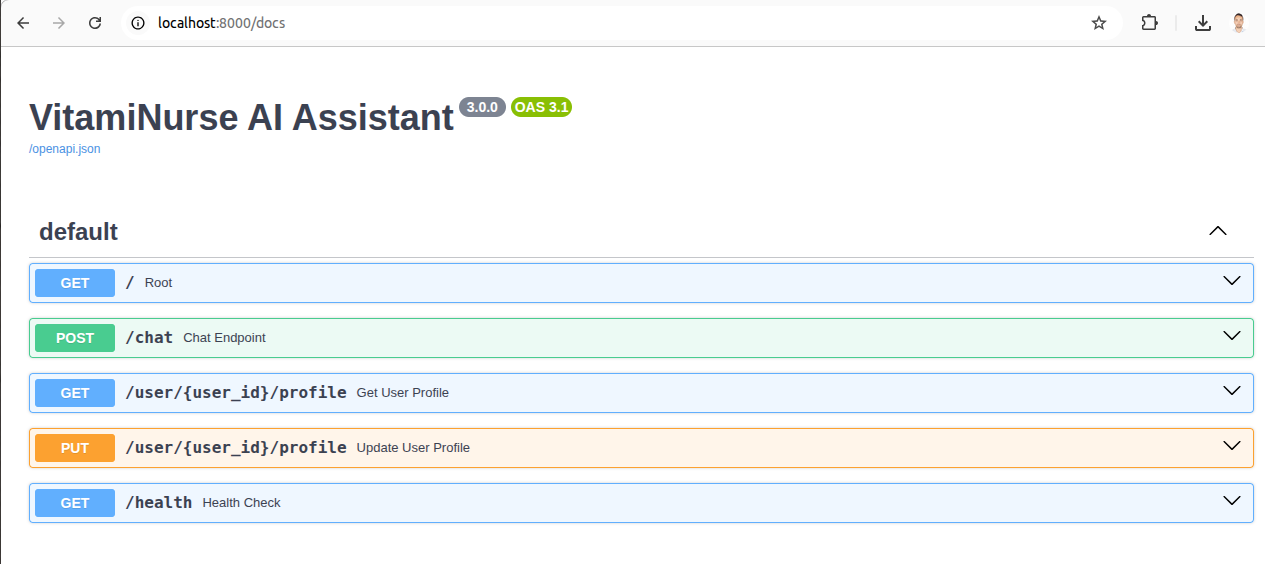
\includegraphics[width=0.9\textwidth]{images/chatbot_API.png}
    \caption{Chatbot FastAPI} 
    \label{fig:chatbot API}
\end{figure}
\end{center}

\newpage
\subsection{AI and Data Layer}
The AI and data layer forms the intelligent core of the VitamiNurse assistant, leveraging advanced language models and sophisticated intent detection to deliver personalized nutritional guidance. At the heart of the system is OpenAI's \texttt{gpt-4o-mini} model, which is meticulously engineered through prompt crafting to provide structured and scientifically grounded nutritional advice.
 \begin{center}
    \begin{figure}[H]
    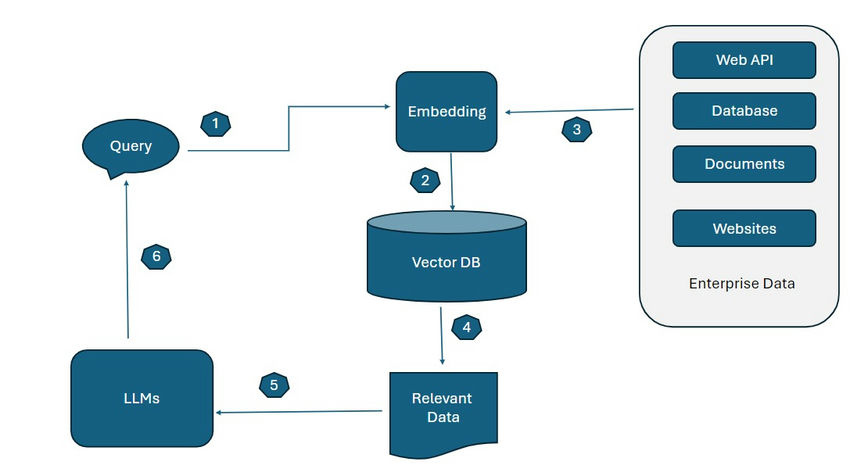
\includegraphics[width=0.9\textwidth]{images/chatbot_ai_data_layer.png}
    \caption{AI and Data Layer in the VitamiNurse Assistant} 
    \label{fig:chatbot_ai_data_layer}
\end{figure}
\end{center}

\subsubsection{Orchestration framework}
The system employs \texttt{LangChain} as its orchestration framework, enabling sophisticated intent detection and parallel processing of user requests. Through LangChain's structured output parsing with Pydantic models, the assistant can simultaneously handle multiple user intents including product searches, recipe generation, profile updates, and general nutritional inquiries.
\subsubsection{Storage layer}
A \texttt{ChromaDB} vector database serves as the persistent storage layer, maintaining semantic embeddings of user profiles, conversation history, and product information. This architecture ensures efficient retrieval and contextual interpretation of information. Moreover, its horizontal scalability guarantees adaptability to evolving user demands.
\subsubsection{Recommendation Engine}
The \emph{recommendation system} introduced in the previous chapter is seamlessly integrated into this architecture. It operates on a hybrid approach combining collaborative filtering and content-based filtering, ensuring that recommended products are both personalized and nutritionally appropriate for each user's specific profile and constraints.

\subsection{Data Organization and Collections}
Data is structured into specialized collections to maximize accessibility and retrieval efficiency. The \textbf{Users Collection} contains individual profiles, including dietary restrictions, health conditions, wellness objectives, and lifestyle preferences, enabling hyper-personalized interactions. The \textbf{Products Collection} indexes items using EAN codes and stores metadata such as nutritional breakdowns, allergen information, and ingredient compositions, allowing rapid identification of suitable food options. 

\subsection{Contextual Knowledge and Guidelines}
The Context Knowledge consists of nutritional cards, each representing a discrete information unit related to health conditions, dietary regimens, or evidence-based guidelines. These cards are periodically updated to reflect current nutritional science. 
Based on these cards, a dynamic nutrition file is constructed and directly utilized by both the recommendation system and the AI assistant to ensure personalized guidance. Furthermore, feature engineering techniques are applied to enrich product data with nutritional labels, thereby enabling more accurate classification and alignment with individual user needs. The implementation is supported by the \texttt{nutrition\_utils.py} module, which specifies ingredients to be avoided for specific users, such as pregnant women or diabetic persons.


\section{Key Features and Implementation}

\subsection{Parallel Intent Processing with LangChain}
\begin{center}
\begin{figure}[H]
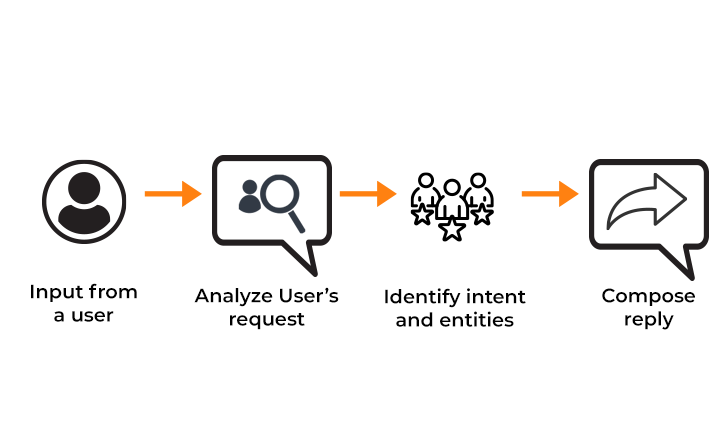
\includegraphics[scale=0.65]{images/how_AI_chatbot_works.png}
\caption{Intent detection and processing in AI chatbots} 
\label{fig:intent_detection}
\end{figure}
\end{center}

A distinctive feature of the VitamiNurse assistant is its ability to process multiple user intents simultaneously using LangChain's parallel processing capabilities, as illustrated in the previous figure. The system employs specialized chains for:
\begin{itemize}
\item \textbf{Product Search}: Detecting product queries and EAN codes, searching ChromaDB, and invoking the recommendation API
\item \textbf{Recipe Generation}: Analyzing culinary preferences and generating personalized recipes using GPT-4
\item \textbf{Profile Management}: Extracting and updating user information from conversational context
\item \textbf{General Queries}: Handling nutritional questions and educational content
\end{itemize}

This parallel architecture ensures that users receive comprehensive responses addressing all aspects of their queries without sequential processing delays.

\subsection{Dynamic Updating of User Profiles}
The assistant's personalization engine is driven by an intelligently evolving user profile defined through Pydantic models. The system automatically extracts and updates profile information from natural conversations using GPT-4's extraction capabilities. Key profile attributes include:
\begin{itemize}
\item Dietary restrictions and allergies
\item Health conditions and medical considerations
\item Nutritional goals and preferences
\item Pregnancy status and special requirements
\item Favorite foods and taste preferences
\end{itemize}

The profile management system employs smart merging strategies that only update changed information while preserving existing valid data. This dynamic updating occurs in real-time during conversations, allowing the assistant to immediately incorporate new user information into its recommendations.
\begin{center}
\begin{figure}[H]
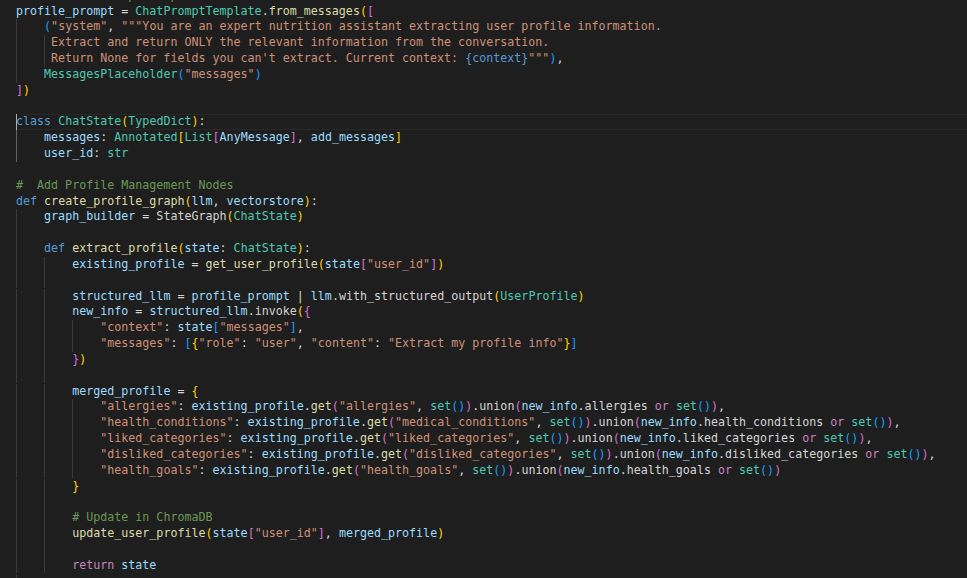
\includegraphics[width=0.9\textwidth]{images/update_user_profile.png}
\caption{Intelligent user profile update through conversational extraction}
\label{fig:user_update_profile}
\end{figure}
\end{center}

\subsection{AI-Powered Recipe Generation}
The system features an advanced recipe generation capability that creates personalized meal suggestions based on multiple factors:
\begin{itemize}
\item User's dietary restrictions and allergies
\item Detected cuisine preferences from conversation
\item Nutritional requirements and health goals
\ ingredient availability and preparation complexity
\end{itemize}

Recipes are generated entirely by GPT-4 and structured into standardized JSON format containing complete nutritional information, preparation steps, cooking times, and customization suggestions. This approach ensures recipes are both personalized and practical for everyday use.

\subsection{Integrated Recommendation System}
The recommendation engine works in concert with the conversational AI to provide context-aware product suggestions. The integration follows a sophisticated workflow:
\begin{enumerate}
\item Intent detection identifies product-related queries
\item ChromaDB performs semantic search for relevant products
\item The recommendation API processes user-specific constraints
\item Results are filtered based on dietary rules and nutritional quality
\item GPT-4 generates natural language explanations of recommendations
\end{enumerate}

This seamless integration ensures that product recommendations are not only relevant to the search query but also safe and appropriate for the user's specific health profile and nutritional needs.

The architecture represents a significant advancement in conversational AI for healthcare applications, demonstrating how LangChain can orchestrate complex multi-intent processing while maintaining coherent, personalized user experiences.

\section{Challenges and Solutions}
Throughout development, several significant challenges emerged in creating a robust conversational nutrition assistant. Maintaining coherent conversation context across extended interactions was addressed through LangChain's sophisticated memory management and ChromaDB's persistent conversation storage. Personalizing recommendations without burdening users with excessive input requirements was solved through GPT-4's intelligent information extraction capabilities, which automatically detect and update user profiles from natural conversation.

Ensuring structured, explainable nutritional advice was achieved through rigorous prompt engineering and Pydantic output parsing, enforcing consistent response formats. Handling ambiguous or incomplete user queries was resolved through the parallel intent processing architecture, which allows multiple interpretation paths to be explored simultaneously before synthesizing a comprehensive response.

The integration of multiple AI components (LangChain chains, GPT-4, ChromaDB, and the recommendation API) presented coordination challenges that were overcome through asynchronous processing patterns and robust error-handling mechanisms.

\section{Future Improvements}
Planned enhancements focus on expanding the assistant's capabilities and integration points. Multi-modal support will enable image-based food recognition and nutritional analysis through advanced computer vision integration. Expanded wearable device connectivity will incorporate real-time physiological data from fitness trackers and health monitors, allowing for dynamic nutritional adjustments based on activity levels and metabolic states.

Advanced personalization through reinforcement learning will enable the system to continuously improve its recommendations based on user feedback and outcomes. Voice interaction capabilities will be enhanced through integration with popular voice assistants (Alexa, Google Assistant) and development of custom voice interfaces for hands-free nutritional guidance.

Additional planned features include:
\begin{itemize}
\item \textbf{Meal Planning Automation}: Multi-day meal planning with grocery list generation
\item \textbf{Social Features}: Community recipe sharing and nutritional challenges
\item \textbf{Healthcare Integration}: EHR connectivity for medical condition management
\item \textbf{Advanced Analytics}: Nutritional intake tracking and trend analysis
\item \textbf{Multi-language Support}: Expansion beyond French to global markets
\end{itemize}


\section{Nodes and Workflow in LangGraph}
The operational backbone of the VitamiNurse AI Assistant is realized through a state machine implemented via LangGraph, a framework that models complex workflows as interconnected nodes with conditional transitions. This design facilitates a modular and traceable execution path, where each node represents a discrete functional unit, contributing to the assistant's responsiveness and adaptability.

\subsection{Intent Classification}
The workflow commences with the \textbf{Classify Intent} node, which analyzes the user's query to categorize it—whether it pertains to product inquiries, recipe suggestions, general nutritional information, health analyses, or profile adjustments. This initial classification ensures that subsequent processing is precisely targeted, optimizing resource utilization.

\subsection{Profile Retrieval}
Following intent detection, the \textbf{Retrieve Profile} node accesses the user's personalized data from ChromaDB. If no profile exists, it initializes a default one, thereby accommodating new users while maintaining continuity for returning ones.

\subsection{Contextual Knowledge Retrieval}
Next, the \textbf{Retrieve Context} node gathers pertinent information from vector databases, such as product details, recipe formulations, or established health guidelines, to enrich the response with accurate and contextually relevant content.

\subsection{Response Generation}
The \textbf{Generate Response} node then employs GPT-4, guided by meticulously crafted prompts, to synthesize a personalized, evidence-based reply that prioritizes user safety and nutritional accuracy.

\subsection{Profile Update Extraction}
In parallel or sequentially, depending on the query, the \textbf{Extract Profile Updates} node scans the conversation for novel information, such as newly disclosed allergies or shifting dietary preferences, extracting actionable insights.

\subsection{Profile Persistence}
If updates are identified, the \textbf{Update Profile} node persists these changes back to ChromaDB, ensuring that the user's profile evolves dynamically over time.

\subsection{Conditional Routing and State Management}
LangGraph's conditional routing enhances this workflow; for example, when new health data emerges, the system diverts the process through extraction and update nodes before finalizing the response. This stateful orchestration not only streamlines interactions but also imbues the assistant with a sense of memory and progression, akin to a human nutritionist's ongoing relationship with a client.

\section{User Profile Management}

\subsection{Profile Initialization}
New users are onboarded through a guided registration process, during which a default profile is created with baseline attributes such as age, gender, dietary preferences, and health objectives. This initial setup allows the VitamiNurse assistant to provide relevant recommendations immediately while accommodating progressive personalization as the user interacts with the system.

\subsection{Profile Evolution}
User profiles are dynamically updated based on interactions, such as conversational inputs, reported allergies, or changes in health conditions. The assistant continuously refines recommendations by integrating these updates, ensuring that dietary advice remains aligned with evolving user needs and goals.

\subsection{Preference Management}
Users can explicitly define or adjust preferences, including favored cuisines, meal frequency, or specific nutrient targets. Preference management allows the assistant to tailor recipe suggestions and nutritional guidance more accurately, enhancing user engagement and satisfaction.

\subsection{Allergy and Dietary Restriction Handling}
The system tracks and enforces dietary restrictions and allergen information. Whenever a new restriction is added, the assistant automatically filters out incompatible products and recipes, maintaining safety and compliance with individual health requirements.

\subsection{Profile Security and Privacy}
User profiles are protected via secure authentication and access control mechanisms, with sensitive information safeguarded against unauthorized access. In the context of VitamiNurse, AWS Cognito manages user authentication, ensuring that only verified users can access or modify personal data. This security layer maintains privacy while allowing the assistant to provide personalized guidance.


\section{Technologies Used}
The VitamiNurse AI Assistant amalgamates a suite of advanced technologies, each selected for its prowess in enabling intelligent, scalable, and secure nutritional advising. This technological synergy forms the foundation for the assistant's sophisticated capabilities.

\subsection{FastAPI for Web Services}
\textbf{FastAPI} undergirds the web interface, offering a high-performance framework for RESTful endpoints that handle real-time user interactions with minimal latency and robust error handling. Its asynchronous design ensures scalability, making it well-suited for handling multiple concurrent users.

\subsection{LangChain for Orchestration}
\textbf{LangChain} facilitates the orchestration of language model invocations, incorporating structured prompting and contextual reasoning chains to weave together complex reasoning processes. This layer ensures coherent integration between data retrieval, reasoning, and response generation.

\subsection{GPT-4 as Core Language Model}
At the heart of the system is \textbf{GPT-4}, OpenAI's flagship large language model, which excels in comprehending nuanced user inputs and generating coherent, context-aware recommendations grounded in vast pre-trained knowledge. Its adaptability allows precise alignment with nutritional and healthcare contexts.

\subsection{Prompt Engineering for Safety and Personalization}
\textbf{Prompt Engineering} plays a pivotal role, with prompts meticulously engineered to enforce safety protocols, personalize outputs, and maintain factual accuracy. This mitigates risks inherent in AI-generated health advice, ensuring responses are reliable, ethically sound, and user-specific.

\subsection{ChromaDB for Long-Term Memory}
\textbf{ChromaDB} provides the vector storage backbone, supporting similarity-based retrievals that endow the assistant with long-term memory for users, products, and recipes alike. This persistent memory enables contextual continuity across interactions, enhancing personalization.

\subsection{StateGraph from LangGraph for Workflow Management}
\textbf{StateGraph}, a module within LangGraph, structures the workflows into modular nodes with dynamic transitions. It enables the assistant’s logic to remain both extensible and comprehensible, ensuring transparent execution paths and robust state management.

\subsection{Technological Synergy}
Collectively, these technologies converge to create an ecosystem that is not only technically proficient but also aligned with ethical standards in AI-assisted healthcare. Their integration ensures a balance between performance, personalization, and trustworthiness in user-facing interactions.

\section{Scenarios of Interaction}
To illustrate the practical efficacy of the VitamiNurse AI Assistant, consider several representative interaction scenarios that highlight its adaptive and user-centric functionality.

\subsection{Recipe Recommendations for Health Conditions}
In one scenario, a user inquires, "Suggest recipes for someone with diabetes." The assistant first retrieves the user's profile to incorporate any pre-existing preferences or restrictions. It then queries the Recipes Collection in ChromaDB, applying filters for diabetic suitability, and generates a curated list of recipes complete with nutritional analyses and preparation steps, ensuring alignment with evidence-based guidelines.

\subsection{Profile Updates and Adaptive Learning}
Another common interaction involves profile updates, such as when a user states, "I am allergic to peanuts." The system classifies this as an update intent, extracts the allergy detail, and integrates it into the user's profile in ChromaDB. Subsequent recommendations automatically exclude peanut-containing items, demonstrating the assistant's capacity for learning and adaptation over time.

\subsection{Product-Oriented Queries for Nutritional Choices}
For product-oriented queries, like "Find me healthy snacks under 200 calories," the assistant searches the Products Collection, cross-referencing with the user's goals and presents options with detailed breakdowns of calories, macronutrients, and health benefits, empowering informed choices.

\subsection{Versatility and Personalization}
These scenarios underscore the assistant's versatility, transforming abstract queries into tangible, personalized support that evolves with user input. The ability to shift seamlessly between recipes, product searches, and profile management highlights its role as a dynamic nutritional companion.


\section{Future Improvements}
Planned enhancements include support for multi-modal inputs, such as image-based food logging and improved barcode scanning accuracy; integration with wearable health devices for real-time physiological monitoring; reinforcement learning approaches to refine personalization over time; and voice-based interaction compatibility with popular assistants such as Alexa and Google Assistant.

\section{Conclusion}
The VitamiNurse AI Nutrition Assistant successfully integrates the capabilities of the Recommendation Engine from the previous chapter into a fully conversational, context-aware platform for personalized dietary guidance. By combining long-term conversational memory, dynamic profile adaptation, and structured prompt engineering, it delivers precise, explainable, and actionable nutritional advice. This positions VitamiNurse as a powerful tool in digital health, with future expansions aimed at real-time adaptability and multimodal engagement. Future enhancements could further amplify its impact, such as integrating real-time health data from wearables, thereby advancing the frontier of AI in personalized nutrition.
